\section{Sperren 2}

Grundlage dieser Aufgabe ist ein Datenbanksystem, das Serialisierbarkeit durch Sperren sicherstellt. Es verwendet dabei S-Sperren (shared locks), X-Sperren (eXclusive locks), IS-Sperren (intention shared locks), IX-Sperren (intention exclusive locks) und SIX-Sperren (shared and intention exclusive locks).

Die Datenobjekte sind folgendermaßen hierarchisch organisiert:

\begin{center}
	\colorbox{white}{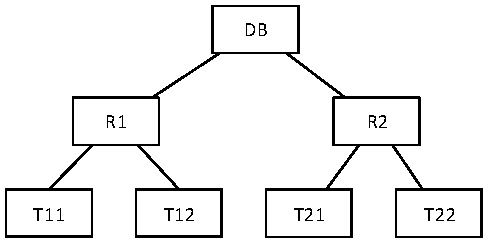
\includegraphics{Pictures/UeIDB14_Sperrhierarchie.pdf}}
\end{center}
\begin{normalText}
\begin{itemize}
	\item Geben Sie für jeden der unten genannten Abläufe an, ob Probleme auftreten, wenn der Ablauf ohne Sperren ausgeführt wird, und wenn ja, welche.
	\item Führen Sie die Abläufe jeweils wie in Aufgabe \ref{Sperren} mit einer Sperrtabelle aus.
\end{itemize}
Zur Vereinfachung können Sie folgende Sperrtabelle verwenden:

\begin{tabular}{|c|c|c|c|c|c|}
	\hline
	Objekte $\backslash$ Sperren & IS & IX & S & SIX & X \\ \hline
	             DB              &    &    &   &     &   \\ \hline
	             R1              &    &    &   &     &   \\ \hline
	             R2              &    &    &   &     &   \\ \hline
	            T11              &    &    &   &     &   \\ \hline
	            T12              &    &    &   &     &   \\ \hline
	            T21              &    &    &   &     &   \\ \hline
	            T22              &    &    &   &     &   \\ \hline
\end{tabular}

\begin{enumerate}[a)]
	\item
	\begin{note}
		Kennenlernen der Sperrhierarchie:
	\end{note}
	$r_1[T11], r_1[T12], w_1[T12], r_1[R2], r_1[DB], w_1[DB], w_1[T21], c_1$
	\item
	\begin{note}
		Das Phantom Problem:
	\end{note}
	$r_1[R1], w_2[T11], r_2[T21], w_2[T21], r_1[R2], c_1, c_2$
	\item $r_1[R2], w_2[T12], r_3[DB], w_1[T11], w_1[T21], w_2[T11], w_3[R2], c_3, r_2[DB], c_2, c_1$
\end{enumerate}
\end{normalText}

\begin{note}
	\paragraph{\color{notecolor}Hinweis:} \textcolor{blue}{Blau:} wird in diesem Schritt bearbeitet, \textcolor{green}{Grün:} wird aufgrund von nicht erhaltenen Sperren verzögert.

	\begin{enumerate}[a)]
		\item $\textcolor{blue}{r_1[T11]}, r_1[T12], w_1[T12], r_1[R2], r_1[DB], w_1[DB], w_1[T21], c_1$

		Kein Problem, da nur eine Transaktion.

		\begin{tabular}{|c|c|c|c|c|c|}
			\hline
			Objekte $\backslash$ Sperren & IS & IX & S & SIX & X \\
			\hline
			DB & T1 &  &  &  &  \\
			\hline
			R1 & T1 &  &  &  &  \\
			\hline
			R2 &  &  &  &  &  \\
			\hline
			T11 &  &  & T1 &  &  \\
			\hline
			T12 &  &  &  &  &  \\
			\hline
			T21 &  &  &  &  &  \\
			\hline
			T22 &  &  &  &  &  \\
			\hline
		\end{tabular}

	$\textcolor{blue}{r_1[T12]}, w_1[T12], r_1[R2], r_1[DB], w_1[DB], w_1[T21], c_1$

	\begin{tabular}{|c|c|c|c|c|c|}
		\hline
		 & IS & IX & S & SIX & X \\
		\hline
		DB & T1 &  &  &  &  \\
		\hline
		R1 & T1 &  &  &  &  \\
		\hline
		R2 &  &  &  &  &  \\
		\hline
		T11 &  &  & T1 &  &  \\
		\hline
		T12 &  &  & T1 &  &  \\
		\hline
		T21 &  &  &  &  &  \\
		\hline
		T22 &  &  &  &  &  \\
		\hline
	\end{tabular}

	$\textcolor{blue}{w_1[T12]}, r_1[R2], r_1[DB], w_1[DB], w_1[T21], c_1$

		\begin{tabular}{|c|c|c|c|c|c|}
		\hline
		& IS & IX & S & SIX & X \\
		\hline
		DB &  & T1 &  &  &  \\
		\hline
		R1 &  & T1 &  &  &  \\
		\hline
		R2 &  &  &  &  &  \\
		\hline
		T11 &  &  & T1 &  &  \\
		\hline
		T12 &  &  &  &  & T1 \\
		\hline
		T21 &  &  &  &  &  \\
		\hline
		T22 &  &  &  &  &  \\
		\hline
	\end{tabular}

	$\textcolor{blue}{r_1[R2]}, r_1[DB], w_1[DB], w_1[T21], c_1$

\begin{tabular}{|c|c|c|c|c|c|}
	\hline
	& IS & IX & S & SIX & X \\
	\hline
	DB &  & T1 &  &  &  \\
	\hline
	R1 &  & T1 &  &  &  \\
	\hline
	R2 &  &  & T1 &  &  \\
	\hline
	T11 &  &  & T1 &  &  \\
	\hline
	T12 &  &  &  &  & T1 \\
	\hline
	T21 &  &  &  &  &  \\
	\hline
	T22 &  &  &  &  &  \\
	\hline
\end{tabular}

	$\textcolor{blue}{r_1[DB]}, w_1[DB], w_1[T21], c_1$

\begin{tabular}{|c|c|c|c|c|c|}
	\hline
	& IS & IX & S & SIX & X \\
	\hline
	DB &  &  &  & T1 &  \\
	\hline
	R1 &  & T1 &  &  &  \\
	\hline
	R2 &  &  & T1 &  &  \\
	\hline
	T11 &  &  & T1 &  &  \\
	\hline
	T12 &  &  &  &  & T1 \\
	\hline
	T21 &  &  &  &  &  \\
	\hline
	T22 &  &  &  &  &  \\
	\hline
\end{tabular}

	$\textcolor{blue}{w_1[DB]}, w_1[T21], c_1$

\begin{tabular}{|c|c|c|c|c|c|}
	\hline
	& IS & IX & S & SIX & X \\
	\hline
	DB &  &  &  &  & T1 \\
	\hline
	R1 &  & T1 &  &  &  \\
	\hline
	R2 &  &  & T1 &  &  \\
	\hline
	T11 &  &  & T1 &  &  \\
	\hline
	T12 &  &  &  &  & T1 \\
	\hline
	T21 &  &  &  &  &  \\
	\hline
	T22 &  &  &  &  &  \\
	\hline
\end{tabular}

	$\textcolor{blue}{w_1[T21]}, c_1$

\begin{tabular}{|c|c|c|c|c|c|}
	\hline
	& IS & IX & S & SIX & X \\
	\hline
	DB &  &  &  &  & T1 \\
	\hline
	R1 &  & T1 &  &  &  \\
	\hline
	R2 &  &  &  & T1 &  \\
	\hline
	T11 &  &  & T1 &  &  \\
	\hline
	T12 &  &  &  &  & T1 \\
	\hline
	T21 &  &  &  &  & T1 \\
	\hline
	T22 &  &  &  &  &  \\
	\hline
\end{tabular}

	$\textcolor{blue}{c_1}$

\begin{tabular}{|c|c|c|c|c|c|}
	\hline
	 & IS & IX & S & SIX & X \\
	\hline
	DB &  &  &  &  &  \\
	\hline
	R1 &  &  &  &  &  \\
	\hline
	R2 &  &  &  &  &  \\
	\hline
	T11 &  &  &  &  &  \\
	\hline
	T12 &  &  &  &  &  \\
	\hline
	T21 &  &  &  &  &  \\
	\hline
	T22 &  &  &  &  &  \\
	\hline
\end{tabular}

\item $\textcolor{blue}{r_1[R1]}, w_2[T11], r_2[T21], w_2[T21], r_1[R2], c_1, c_2$

Problem: Ja, Phantom Problem

\begin{tabular}{|c|c|c|c|c|c|}
	\hline
	& IS & IX & S & SIX & X \\
	\hline
	DB & T1 &  &  &  &  \\
	\hline
	R1 &  &  & T1 &  &  \\
	\hline
	R2 &  &  &  &  &  \\
	\hline
	T11 &  &  &  &  &  \\
	\hline
	T12 &  &  &  &  &  \\
	\hline
	T21 &  &  &  &  &  \\
	\hline
	T22 &  &  &  &  &  \\
	\hline
\end{tabular}

$\textcolor{green}{w_2[T11], r_2[T21], w_2[T21]}, \textcolor{blue}{r_1[R2]}, c_1, c_2$

T2 wird blockiert, da R1 bereits von T1 auf S gesperrt ist.

\begin{tabular}{|c|c|c|c|c|c|}
	\hline
	& IS & IX & S & SIX & X \\
	\hline
	DB & T1 &  &  &  &  \\
	\hline
	R1 &  &  & T1 &  &  \\
	\hline
	R2 &  &  & T1 &  &  \\
	\hline
	T11 &  &  &  &  &  \\
	\hline
	T12 &  &  &  &  &  \\
	\hline
	T21 &  &  &  &  &  \\
	\hline
	T22 &  &  &  &  &  \\
	\hline
\end{tabular}

$\textcolor{green}{w_2[T11], r_2[T21], w_2[T21]}, \textcolor{blue}{c_1}, c_2$

T1 committet, die Sperren werden aufgeräumt.

\begin{tabular}{|c|c|c|c|c|c|}
	\hline
	& IS & IX & S & SIX & X \\
	\hline
	DB &  &  &  &  &  \\
	\hline
	R1 &  &  &  &  &  \\
	\hline
	R2 &  &  &  &  &  \\
	\hline
	T11 &  &  &  &  &  \\
	\hline
	T12 &  &  &  &  &  \\
	\hline
	T21 &  &  &  &  &  \\
	\hline
	T22 &  &  &  &  &  \\
	\hline
\end{tabular}

$\textcolor{blue}{w_2[T11]}, r_2[T21], w_2[T21], c_2$

\begin{tabular}{|c|c|c|c|c|c|}
	\hline
	& IS & IX & S & SIX & X \\
	\hline
	DB &  & T2 &  &  &  \\
	\hline
	R1 &  & T2 &  &  &  \\
	\hline
	R2 &  &  &  &  &  \\
	\hline
	T11 &  &  &  &  & T2 \\
	\hline
	T12 &  &  &  &  &  \\
	\hline
	T21 &  &  &  &  &  \\
	\hline
	T22 &  &  &  &  &  \\
	\hline
\end{tabular}

$\textcolor{blue}{r_2[T21]}, w_2[T21], c_2$

\begin{tabular}{|c|c|c|c|c|c|}
	\hline
	& IS & IX & S & SIX & X \\
	\hline
	DB &  & T2 &  &  &  \\
	\hline
	R1 &  & T2 &  &  &  \\
	\hline
	R2 & T2 &  &  &  &  \\
	\hline
	T11 &  &  &  &  & T2 \\
	\hline
	T12 &  &  &  &  &  \\
	\hline
	T21 &  &  & T2 &  &  \\
	\hline
	T22 &  &  &  &  &  \\
	\hline
\end{tabular}

$\textcolor{blue}{w_2[T21]}, c_2$

\begin{tabular}{|c|c|c|c|c|c|}
	\hline
	& IS & IX & S & SIX & X \\
	\hline
	DB &  & T2 &  &  &  \\
	\hline
	R1 &  & T2 &  &  &  \\
	\hline
	R2 &  & T2 &  &  &  \\
	\hline
	T11 &  &  &  &  & T2 \\
	\hline
	T12 &  &  &  &  &  \\
	\hline
	T21 &  &  &  &  & T2 \\
	\hline
	T22 &  &  &  &  &  \\
	\hline
\end{tabular}

$\textcolor{blue}{c_2}$

\begin{tabular}{|c|c|c|c|c|c|}
	\hline
	& IS & IX & S & SIX & X \\
	\hline
	DB &  &  &  &  &  \\
	\hline
	R1 &  &  &  &  &  \\
	\hline
	R2 &  &  &  &  &  \\
	\hline
	T11 &  &  &  &  &  \\
	\hline
	T12 &  &  &  &  &  \\
	\hline
	T21 &  &  &  &  &  \\
	\hline
	T22 &  &  &  &  &  \\
	\hline
\end{tabular}

\item $\textcolor{blue}{r_1[R2]}, w_2[T12], r_3[DB], w_1[T11], w_1[T21], w_2[T11], w_3[R2], c_3, r_2[DB], c_2, c_1$

Probleme: Ja, viele. Mag jetzt nicht nachschauen, welche das alles sind. Evtl.\ anhand der Abgaben ergänzen.

\begin{tabular}{|c|c|c|c|c|c|}
	\hline
	& IS & IX & S & SIX & X \\
	\hline
	DB & T1 &  &  &  &  \\
	\hline
	R1 &  &  &  &  &  \\
	\hline
	R2 &  &  & T1 &  &  \\
	\hline
	T11 &  &  &  &  &  \\
	\hline
	T12 &  &  &  &  &  \\
	\hline
	T21 &  &  &  &  &  \\
	\hline
	T22 &  &  &  &  &  \\
	\hline
\end{tabular}

$\textcolor{blue}{w_2[T12]}, r_3[DB], w_1[T11], w_1[T21], w_2[T11], w_3[R2], c_3, r_2[DB], c_2, c_1$

\begin{tabular}{|c|c|c|c|c|c|}
	\hline
	& IS & IX & S & SIX & X \\
	\hline
	DB & T1 & T2 &  &  &  \\
	\hline
	R1 &  & T2 &  &  &  \\
	\hline
	R2 &  &  & T1 &  &  \\
	\hline
	T11 &  &  &  &  &  \\
	\hline
	T12 &  &  &  &  & T2 \\
	\hline
	T21 &  &  &  &  &  \\
	\hline
	T22 &  &  &  &  &  \\
	\hline
\end{tabular}

$\textcolor{green}{r_3[DB]}, \textcolor{blue}{w_1[T11]}, w_1[T21], w_2[T11], w_3[R2], c_3, r_2[DB], c_2, c_1$

T3 bekommt die Sperre nicht (wegen IX von T1, T2 auf DB).

\begin{tabular}{|c|c|c|c|c|c|}
	\hline
	& IS & IX & S & SIX & X \\
	\hline
	DB & & T2, T1 &  &  &  \\
	\hline
	R1 &  & T2, T1 &  &  &  \\
	\hline
	R2 &  &  & T1 &  &  \\
	\hline
	T11 &  &  &  &  & T1 \\
	\hline
	T12 &  &  &  &  & T2 \\
	\hline
	T21 &  &  &  &  &  \\
	\hline
	T22 &  &  &  &  &  \\
	\hline
\end{tabular}

$\textcolor{green}{r_3[DB]}, \textcolor{blue}{w_1[T21]}, w_2[T11], w_3[R2], c_3, r_2[DB], c_2, c_1$

\begin{tabular}{|c|c|c|c|c|c|}
	\hline
	& IS & IX & S & SIX & X \\
	\hline
	DB & & T2, T1 &  &  &  \\
	\hline
	R1 &  & T2, T1 &  &  &  \\
	\hline
	R2 &  &  &  & T1 &  \\
	\hline
	T11 &  &  &  &  & T1 \\
	\hline
	T12 &  &  &  &  & T2 \\
	\hline
	T21 &  &  &  &  & T1 \\
	\hline
	T22 &  &  &  &  &  \\
	\hline
\end{tabular}

$\textcolor{green}{r_3[DB], w_2[T11], w_3[R2], c_3, r_2[DB], c_2,}\textcolor{blue}{c_1}$

T2 bekommt die Sperre nicht (wegen X von T1 auf T11). T1 committet.

\begin{tabular}{|c|c|c|c|c|c|}
	\hline
	& IS & IX & S & SIX & X \\
	\hline
	DB & & T2&  &  &  \\
	\hline
	R1 &  & T2 &  &  &  \\
	\hline
	R2 &  &  &  &  &  \\
	\hline
	T11 &  &  &  &  &  \\
	\hline
	T12 &  &  &  &  & T2 \\
	\hline
	T21 &  &  &  &  &  \\
	\hline
	T22 &  &  &  &  &  \\
	\hline
\end{tabular}

$\textcolor{green}{r_3[DB]}, \textcolor{blue}{w_2[T11]}, w_3[R2], c_3, r_2[DB], c_2$

T3 ist weiterhin blockiert, T2 darf weiterlaufen.

\begin{tabular}{|c|c|c|c|c|c|}
	\hline
	& IS & IX & S & SIX & X \\
	\hline
	DB & & T2&  &  &  \\
	\hline
	R1 &  & T2 &  &  &  \\
	\hline
	R2 &  &  &  &  &  \\
	\hline
	T11 &  &  &  &  & T2 \\
	\hline
	T12 &  &  &  &  & T2 \\
	\hline
	T21 &  &  &  &  &  \\
	\hline
	T22 &  &  &  &  &  \\
	\hline
\end{tabular}

$\textcolor{green}{r_3[DB], w_3[R2], c_3}, \textcolor{blue}{r_2[DB]}, c_2$

\begin{tabular}{|c|c|c|c|c|c|}
	\hline
	& IS & IX & S & SIX & X \\
	\hline
	DB & & &  & T2 &  \\
	\hline
	R1 &  & T2 &  &  &  \\
	\hline
	R2 &  &  &  &  &  \\
	\hline
	T11 &  &  &  &  & T2 \\
	\hline
	T12 &  &  &  &  & T2 \\
	\hline
	T21 &  &  &  &  &  \\
	\hline
	T22 &  &  &  &  &  \\
	\hline
\end{tabular}

$\textcolor{blue}{r_3[DB]}, w_3[R2], c_3$

T2 committet, T3 darf weiterlaufen.

\begin{tabular}{|c|c|c|c|c|c|}
	\hline
	& IS & IX & S & SIX & X \\
	\hline
	DB &  &  & T3 &  &  \\
	\hline
	R1 &  &  &  &  &  \\
	\hline
	R2 &  &  &  &  &  \\
	\hline
	T11 &  &  &  &  &  \\
	\hline
	T12 &  &  &  &  &  \\
	\hline
	T21 &  &  &  &  &  \\
	\hline
	T22 &  &  &  &  &  \\
	\hline
\end{tabular}

$\textcolor{blue}{w_3[R2]}, c_3$

\begin{tabular}{|c|c|c|c|c|c|}
	\hline
	& IS & IX & S & SIX & X \\
	\hline
	DB &  &  &  & T3 &  \\
	\hline
	R1 &  &  &  &  &  \\
	\hline
	R2 &  &  &  &  & T3 \\
	\hline
	T11 &  &  &  &  &  \\
	\hline
	T12 &  &  &  &  &  \\
	\hline
	T21 &  &  &  &  &  \\
	\hline
	T22 &  &  &  &  &  \\
	\hline
\end{tabular}

$\textcolor{blue}{c_3}$

\begin{tabular}{|c|c|c|c|c|c|}
	\hline
	& IS & IX & S & SIX & X \\
	\hline
	DB &  &  &  &  &  \\
	\hline
	R1 &  &  &  &  &  \\
	\hline
	R2 &  &  &  &  &  \\
	\hline
	T11 &  &  &  &  &  \\
	\hline
	T12 &  &  &  &  &  \\
	\hline
	T21 &  &  &  &  &  \\
	\hline
	T22 &  &  &  &  &  \\
	\hline
\end{tabular}

\end{enumerate}
\end{note}
